\subsection{Solución actividad 4}
\noindent \textbf{Actividad 4}\\
 En la figura 31 se observa un diagrama simplificado del sistema de suspensión en una llanta de un automóvil, mediante la metodología de diseño estudiado obtener el modelo matemático del sistema de suspensión especificando las variables físicas, los elementos almacenadores de flujo, esfuerzo, disipadores y fuentes.\\
Una vez obtenido el modelo matemático defina los parámetros de sistema de suspensión considerando que la masa de un carro es aproximadamente de 2 toneladas y está repartida en las cuatro llantas del automóvil. El objetivo es que los tripulantes sientan lo menos posible las irregularidades de las carreteras. Argumentar su resultado con ayuda de una simulación con matlab.\\
El sistema mostrado consta de las siguientes variables:\\
\begin{itemize}
\item Fuerza de entrada (f(t))
\item Masa (M)
\item Amortiguador (b)
\item Resorte (k)
\item Desplazamiento (x(t)), salida del sistema
\end{itemize}
Los cuales son catalogados de la siguiente manera:
\begin{center}
\begin{tabular}{ c c c c c }
\hline
Almacenador Flujo & Almacenador Esfuerzo & Disipador & Fuente de energía\\
\hline
Masa & Resorte & Amortiguador & Fuerza y el desplazamiento\\
\hline
\end{tabular}
\end{center}
Al ser un sistema mecánico nuestra restricción está presentada por la segunda Ley de Newton:
\begin{equation}
\sum_{n=1}^{\infty}F_i=0
\end{equation}
En nuestro caso, la segunda Ley de Newton aplicada a nuestro sistema tiene la siguiente forma:
\begin{equation}
f(t)=f_k+f_B+f_m
\end{equation}
Sustituyendo las definiciones de cada una de las fuerzas la expresión se transforma a:
\begin{equation}
f(t)=kx+Bv+ma
\end{equation}
Aplicando las definiciones de velocidad y aceleración como la primera derivada y la segunda derivdada del desplazamiento respectivamente llegamos a:
\begin{equation}
f(t)=kx+Bx^{'}+mx^{''}
\end{equation}
Para continuar aplicaremos dos cambios de variables. La entrada va a corresponder a x(t) y la salida a y(t):
\begin{equation}
x(t)=ky(t)+By^{'}(t)+my^{''}(t)
\end{equation}
Si a la ecuación anterior le aplicamos la transformada de laplace en ambos lados llegarmos a la siguiente forma:
\begin{equation}
X(s)=kY(s)+BsY(s)+ms^2Y(s)
\end{equation}
\begin{equation}
X(s)=Y(s)(k+Bs+ms^2)
\end{equation}
Para finalizar usaremos la ecuación anterior para obtener la función de transferencia:
\begin{equation}
\frac{Y(s)}{X(s)}=\frac{1}{(k+Bs+ms^2)}
\end{equation}
Para la simulación y observación de la respuesta del programa se utilizaron los siguientes comandos, tomando en cuenta que el valor de la masa del auto es de dos toneladas y por lo tanto la masa soportada por cada suspensión es de media tonelada:
\begin{verbatim}
H=tf([1],[m B K])
H=tf([1],[500 B K])
step(H,'-')
\end{verbatim}
La respuesta del sistema va a depender de los valores asignados al amortiguador B y al resorte K. Esto nos va a generar cuatro posibles comportamientos:
\begin{itemize}
\item No amortiguado
\item Subamortiguado
\item Criticamente amortiguado
\item Sobreamortiguado
\end{itemize}
Para nuestro diseño nos interesan las últimas dos reacciones, criticamente amortiguado y subamortiguado. Estos comportamientos los lograremos obtener si el valor de el amortiguador (B) es considerablemente mayor al del resorte (k). Si elegimos valores de tal forma en que k sea un $5\%$ del valor de B podemos obtener el comportamiento que deseamos, siendo este el de sobreamortiguado. En la siguiente gráfica se usó un valor de B de dos mil y de k de cien.
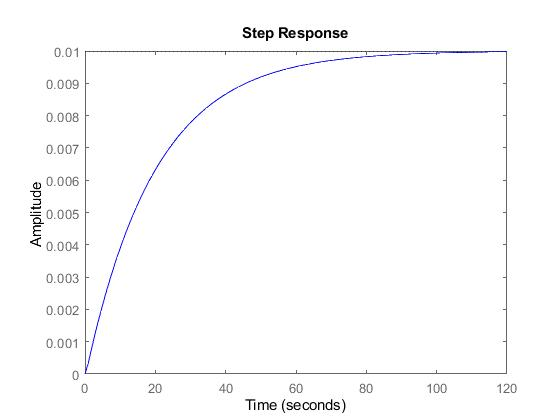
\includegraphics[scale=0.6]{AmortiguadorB2000K100}\\